\section{SOAR}
Heisst: \textbf{Security Orchestration, Automation and Response Solutions}\\

SOAR sammelt ebenfalls Daten aus verschiedenen Quellen, ähnlich wie ein SIEM, aber SOAR unterstützt den Incident Responder bei der Bewältigung der Krise.
SOAR ermöglicht ein automatisiertes Eingreifen, wenn ein Sicherheitsvorfall eintritt.
Ein SOAR-System unterstützt den Incident-Responder auch bei der Einführung von Sicherheitsmaßnahmen (Active Directory).
\begin{itemize}
  \item Untersuchung von Alarmen
  \item Orchestrierung (automatisierte Konfiguration, Verwaltung und Koordinierung)
  \item Automatisierung von Arbeitsabläufen
\end{itemize}

\subsection{SOAR vs. SIEM}
Ein \textbf{SOAR} ermöglicht es dem Sicherheitsteam, die Alerts schnell und effizient zu bewältigen, so dass Zeit für wichtige, fachspezifische Aufgaben bleibt, was zu einem leistungsfähigeren SOC führt.
Ein \textbf{SIEM} sammelt vorallem Daten und generiert Alerts.

\subsection{Velociraptor}
Velociraptor is a unique, advanced open-source endpoint monitoring, digital forensic and cyber response platform.

A powerful DFIR (Digital Forensic and Incident Response) technique is searching bulk data for patterns:
\begin{itemize}
  \item Searching for CC data in process memory
  \item Searching for URLs in process memory
  \item Searching binaries for malware signatures
  \item Searching registry for patterns
\end{itemize}
Bulk searching helps to identify evidence without needing to parse file formats.

\subsection{Virtual File System (VFS)}
\begin{itemize}
  \item \textbf{File}: File system access based on OS FS API
  \item \textbf{NTFS}: NTFS raw parsing filesystem access
  \item \textbf{Registry}: Windows Registry access using the Registry API
  \item \textbf{Artifacts}: Artifacts collected from the client incl. type and time in Velociraptor Artifacts are commands and scripts that actually grab some data (we usually call these artifacts) from clients.
\end{itemize}

\subsubsection{File Download}
You may collect files individually or an entire folder recursively.
Files get marked with the floppy once available on the server.

\subsection{Artifacts}
Velociraptor is a query language engine.
Basically everything is a query (Velociraptor Query Language (VQL)).
Artifacts aim to encapsulate evidence collection:
\begin{itemize}
  \item Structure is YAML
  \item Ideally includes comments
  \item Allow for customization where reasonable
  \item Recursion. Use Artifacts in the query language
\end{itemize}

\subsection{Hunting}
Hunting enables you to collect the same artifacts over an entire fleet.
\begin{itemize}
  \item Only systems that are connected will participate in the hunt
  \item Only systems that are connected will deliver results
  \item Hunts are run for quite some time (days), repeatedly
  \item Hunts may be restricted by label or OS
\end{itemize}

\subsection{Collecting Files}
Incident Response may require for quick conservation of a number artifacts to be analyzed later on or being given somewhere else for analysis. 
With Velociraptor comes the KapeFiles Client Artifact which is a great collector of relevant files.

\paragraph{Approaches}
\begin{itemize}
  \item Run hunt or collection within the Velociraptor Infrastructure
  \item Run standalone collector with Velociraptor
\end{itemize}

\paragraph{What to collect}
Usually good:
\begin{itemize}
  \item \_BasicCollection
  \item \_SANS\_Triage
  \item \_KapeTriage
\end{itemize}

\paragraph{Potential Issues}
Collecting large files will not result in a memory bottleneck as Velociraptor throttles clients if needed. However, extensive hunts on machines or collection of user document folders, virtual machine images, memory dumps could easily jam your servers connection or fill your servers disk. Be careful!

\subsubsection{Download Structure}
\paragraph{Top Level}
The top level includes the hunt configuration details including some meta info.
The client folder contain the results per client workstation name.

\paragraph{Per Client Flow Level}
Within the collections flow folder. The uploaded files are separated by the accessor they got collected with. Thus \$MFT will be available from the ntfs folder. Any common files from the auto folder.

\paragraph{Timestamps and Hashes}
Kape does by default create a VHDX and timestomp files in it. 
So non-tech savvy folks may browse it like a real disk. 
You are better of by using the \$MFT directly.
Timestamps and file hashes in the meta info files.

\subsubsection{Collect manually}
\begin{lstlisting}
  PS C:\> velociraptor.exe artifacts list *Kape*
  Windows.KapeFiles.Targets

  PS C:\> velociraptor.exe artifacts show Windows.KapeFiles.Targets
  parameters:
  ...
  - name: _BasicCollection
    description: "Basic Collection (by Phill Moore): Thumbcache DB, at .job,
    at .job, at SchedLgU.txt, at SchedLgU.txt, XML, XML, LNK Files from Recent, ..."

  PS C:\> velociraptor.exe artifacts collect Windows.KapeFiles.Targets --args=_BasicCollection=Y --output=Collection_$env:computername.zip
\end{lstlisting}

\subsection{Speed}
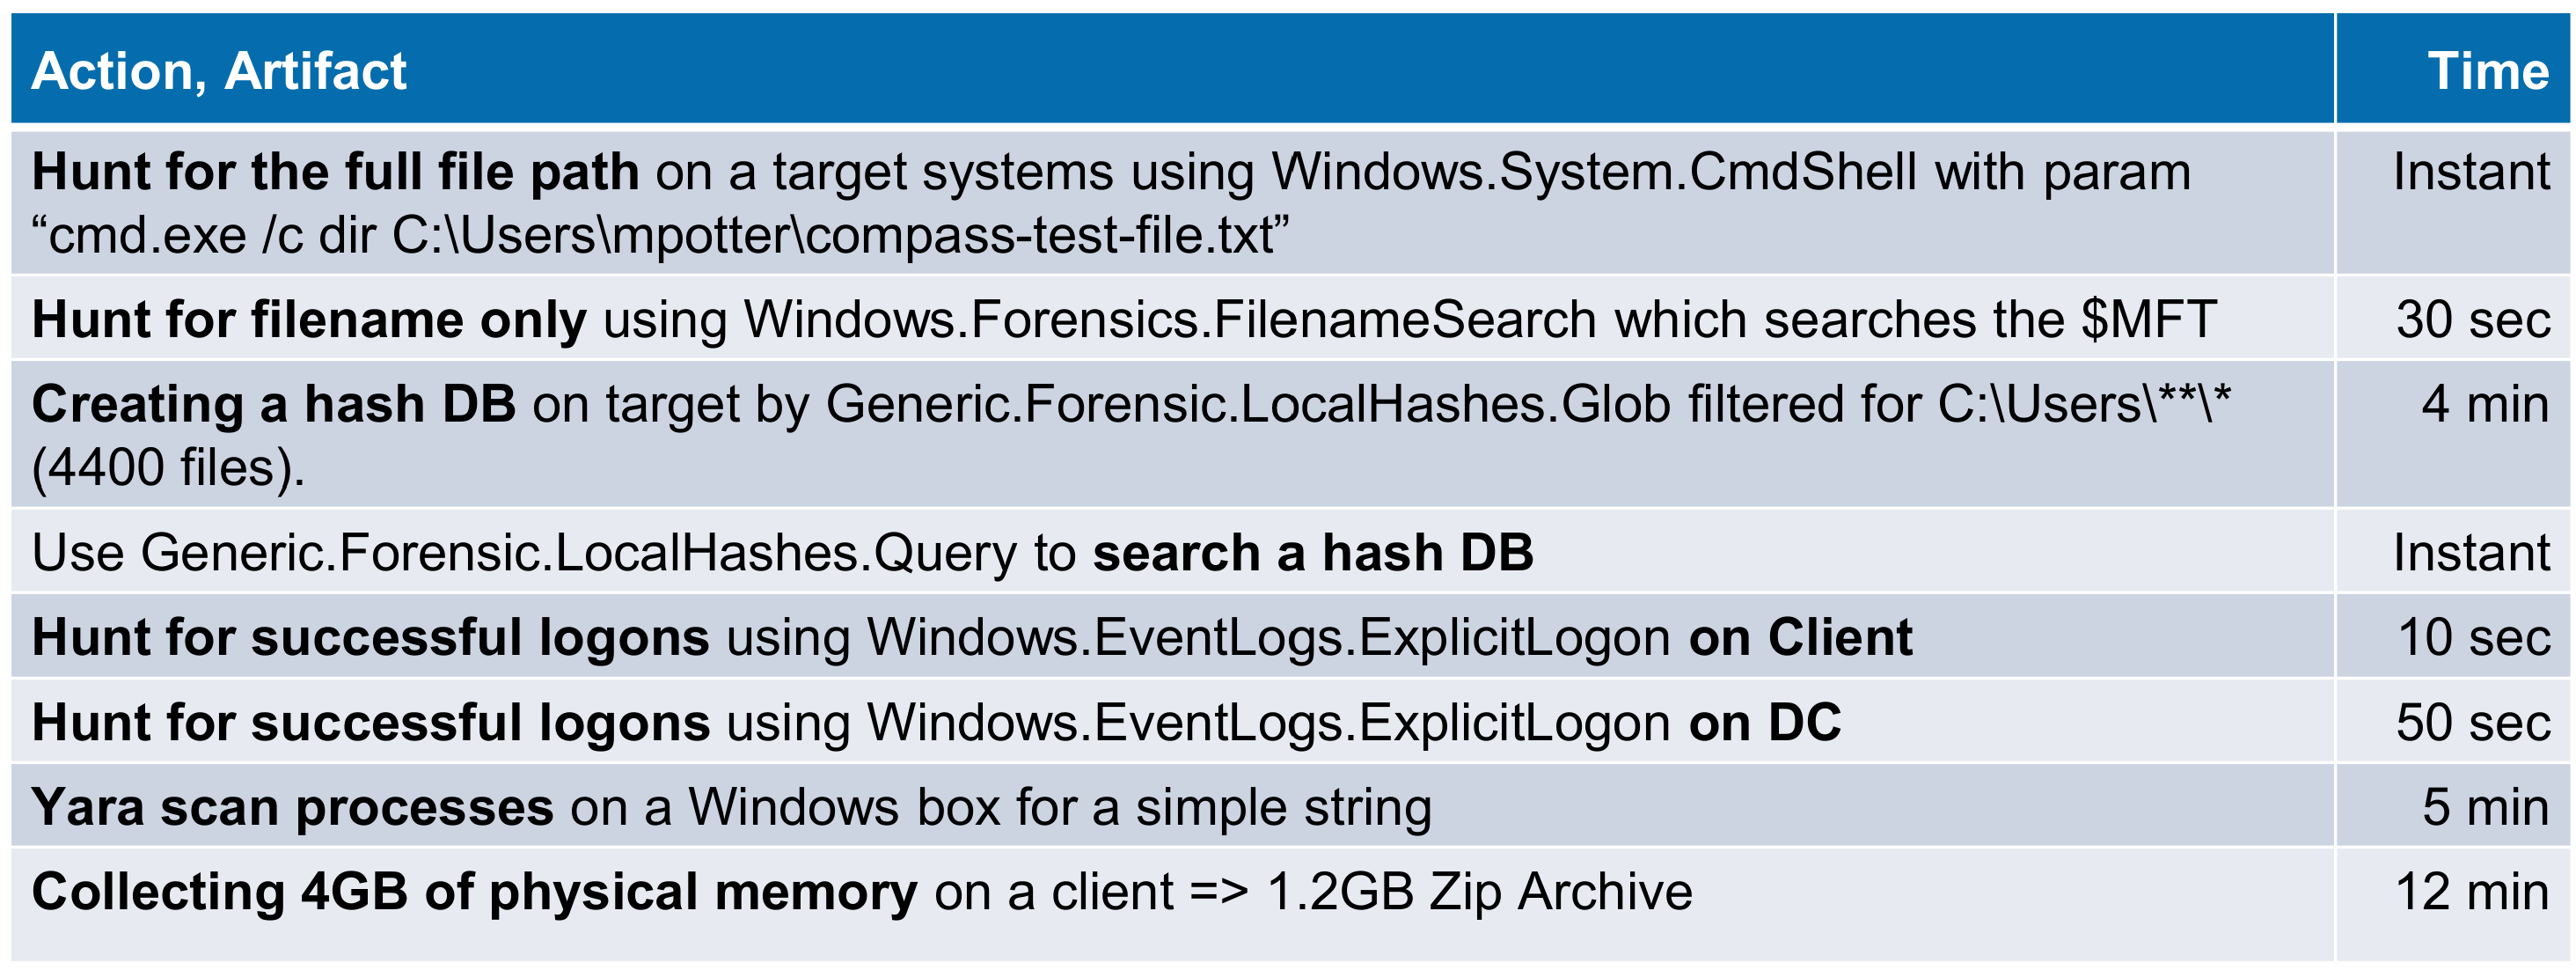
\includegraphics[width=\linewidth]{velociraptor-speed.png}

\subsection{Velociraptor Query Language}
What is VQL:
\begin{itemize}
    \item It looks like SQL
    \item Everything in Velociraptor is basically returning Table (Resultset)
    \item Functions and plugins are the major accelerators
\end{itemize}
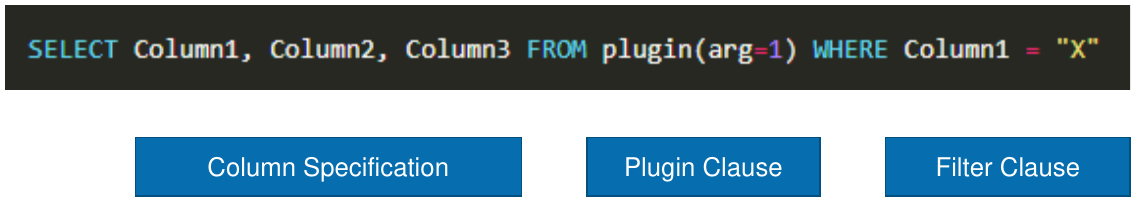
\includegraphics[width=\linewidth]{./img/10-velociraptor/vql.png}

\begin{lstlisting}
-- comment
// comment

#If you want to match strings
SELECT * FROM pslist() WHERE Exe =~ "veloci"

#Put values or entire queries into a variable using LET
LET test = "gugus"
LET test = SELECT * FROM pslist()

#using LIMIT
SELECT * FROM glob(globs="C:/**") LIMIT 5

#Use log() to do Candle-Light Debugging
SELECT Null FROM pslist() WHERE log(message="yeah, hit line")

#Use the glob plugin to get a list of files easily.
SELECT Name FROM glob(globs= "C:/Users/**/Downloads/*.ex?") LIMIT 5

Globs support wildcards such as
? for a single letter
* part of a string
** used to traverse recursively into folder

#Globs support different file accessors e.g. the Registry
SELECT FullPath, Name, Data.type, Data.value FROM glob(globs= "HKEY_USERS/*/Software/**/*", accessor="reg")

#Use if to branch depending on a condition
SELECT * FROM if(
    condition=Exe =~ "chrome",
    then={ expression or query },
    else={ expression or query }
    // else is optional
)

#You may loop over result sets using foreach applying a sub query
LET foo = SELECT * FROM pslist() where Exe =~ "chrome" LIMIT 5
SELECT * FROM foreach(
    row=foo,
    query={SELECT * FROM handles(pid=Pid)}
)

#Create a query that lists loaded DLLs for Velociraptor including compile time and signature
LET pids = SELECT * FROM pslist() WHERE Exe =~ "veloci"
SELECT * FROM foreach( row = pids, query = {
    SELECT Pid, ExePath, parse_pe(file=ExePath) .FileHeader.TimeDateStamp as
    CompileTime, authenticode(filename=ExePath) .SubjectName as Subject,
    authenticode(filename=ExePath) .Trusted as Trusted FROM modules(pid=Pid)
})
\end{lstlisting}

\subsubsection{Registry Search}
Velociraptor can be used to search the registry of a client in several ways
\begin{enumerate}
    \item Manually look through the registry
    \item Design your own VQL query and use the Notebook
    \item Run a hunt on only Forensic to get the information
\end{enumerate}


\subsubsection{Notebook - raw\_reg}
Like the \textit{raw\_reg} accessor, the zip accessor also requires a url. Here is what a query for all files ending with .jpg in the zip file \lstinline|C:\Users\Bob\Desktop\images.zip| could look like:

\begin{lstlisting}[language=bash]
    SELECT * FROM glob(globs=url(scheme='ntfs', path ='C:/Users/Bob/Desktop/images.zip', fragment='/**/*.jpg').String, accessor='zip')
\end{lstlisting}

\subsubsection{Notebook - foreach}
To not only do this for the current user but all users, you have to use a \textit{foreach} plugin.

The following statement would give you the Name and executable path for all executables that are running as the user(s) with the SID that is also running a process that has velociraptor in its executable path.

\begin{lstlisting}[language=bash]
    SELECT * FROM foreach(
    row={SELECT OwnerSid AS velociraptor_owner FROM pslist() WHERE Exe=~'velociraptor'},
    query={SELECT Name, Exe FROM pslist() WHERE OwnerSid=velociraptor_owner}
)
\end{lstlisting}

\subsubsection{Builtin Artifacts}
Velociraptor already comes with a number of pre-built artifacts for frequently needed queries.
This includes for example querying the registry (\lstinline|Windows.Registry.NTUser|).

\subsubsection{YARA Artifact}
You might have to use a foreach loop again where the rows statement gives you the PIDs and names of all processes and then scan for the YARA signature in the query block.





\subsection{Deployment}
Velociraptor will create configuration files from which you can build clients and servers for various architectures (provided the architecture has a compiler for GO available).\\

\subsubsection{Linux}
To build a Linux server Debian installer package on Windows, run
\begin{lstlisting}
  velociraptor.exe config generate -i
  velociraptor.exe --config server.config.yaml debian server
\end{lstlisting}
To install the server deb package on Debian, run:
\begin{lstlisting}
  sudo dpkg -i velociraptor_server*.deb
  sudo server service velociraptor_server status
\end{lstlisting}
Installation of the package might fail due to dependency errors. In that case run apt-get install -f and rerun the above.

\subsubsection{Windows}
To create an .msi installer file. Unzip the Velociraptor source and change to the WIX folder:
\begin{lstlisting}
  cd velociraptor-src\docs\wix
  mkdir output
  copy pathobinary\velociraptor.exe output\velociraptor.exe
  copy pathobinary\client.config.yaml output\
  build_custom.bat
\end{lstlisting}

\paragraph{Information for Windows}
You are strongly advised to sign Windows binaries to avoid hiccups with Defender. Use Microsofts signtool.exe or osslsigncode on Linux.\\

Binaries are usually deployed either by:
\begin{itemize}
  \item GPO scheduled tasks
  \item GPO assigned software
  \item Microsoft System Center Configuration Manager (SCCM)
  \item Some other custom SW deployment mechanism
\end{itemize}

\subsection{Labs - Lateral Movement}
Lateral movement means to move within the internal network to access the organization's target data and to exfiltrate the data. In this challenge you will solve tasks to detect lateral movement using Velociraptor.

\subsubsection{Detection PsExec}
To Detect if someone used \textit{PsExec} after passing the hash, there are multiple ways. One way is to design your own Artifact based on \lstinline|Windows.Registry.Sysinternals.Eulacheck| Artifact.

\subsubsection{Use Velociraptor Artifact}
In Velociraptor, use the Artifact \lstinline|Windows.EventLogs.AlternateLogon|. It will list all Windows events with ID \textit{4648}. Use the timestamp function from Velociraptor to change the timestamp to date time format.

\subsubsection{Event Correlation}
With the event results from the Artifacts used, do an event correlation by matching the time at which both events occurred. Both event should have a temporal correlation.

\subsubsection{Evidence on Destination}
As you will see in the result of Artifact \lstinline|Windows.EventLogs.AlternateLogon|, the TargetServerName was DC1. Look for evidence of execution on destination DC1 by searching for event ID \textit{4624} as mentioned in SANS Hunt Evil Poster.

\subsubsection{Detection Mimikatz}
Now you have collected some evidence that someone did misuse \textit{PsExec} for passing the hash. But to dump the hash from a node, you need a tool. One such tool is Mimikatz. Use the \lstinline|Windows.System.Amcache| Artifact to detect if Mimikatz was executed on the system.